\documentclass{article}
\usepackage[utf8]{inputenc}
\usepackage{xcolor}
\usepackage{graphicx}
\title{BME 646/ ECE695DL: Homework 2}
\author{Chengjun Guo} 
\date{24 January 2022}


\begin{document}
\maketitle
\section{Introduction}
This homework is to open image file as PIL object and process it with a combination of numpy and PyTorch functions.
\section{Methodology}
In this homework, I used totensor, normalize, compose from torchvision.transform and to convert the image into normalized tensor. Then I defined $task3_4func$ that would include channel based histogram and normalization, histogram plotting from pyplot and wasserstein distance calculating. Then I did the same process to the affined image and perspective image.

\section{Implementation and Results}
\subsection{printed figures}
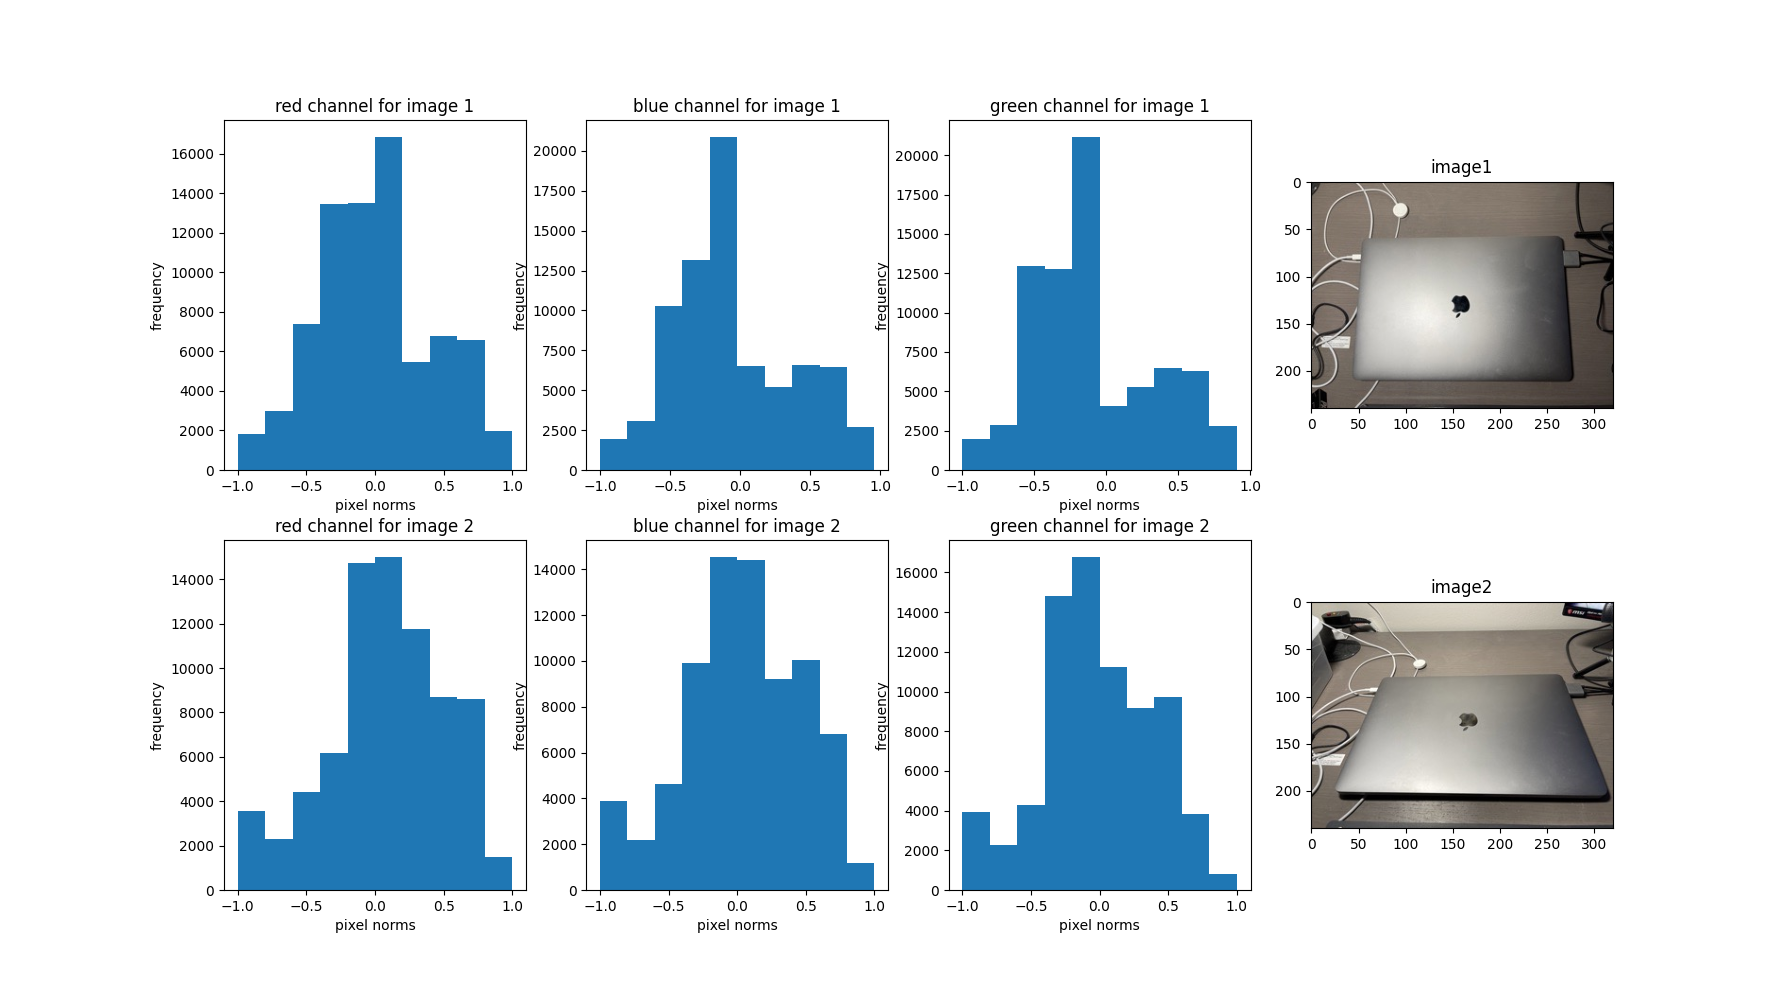
\includegraphics[scale=0.38]{1.png}\\
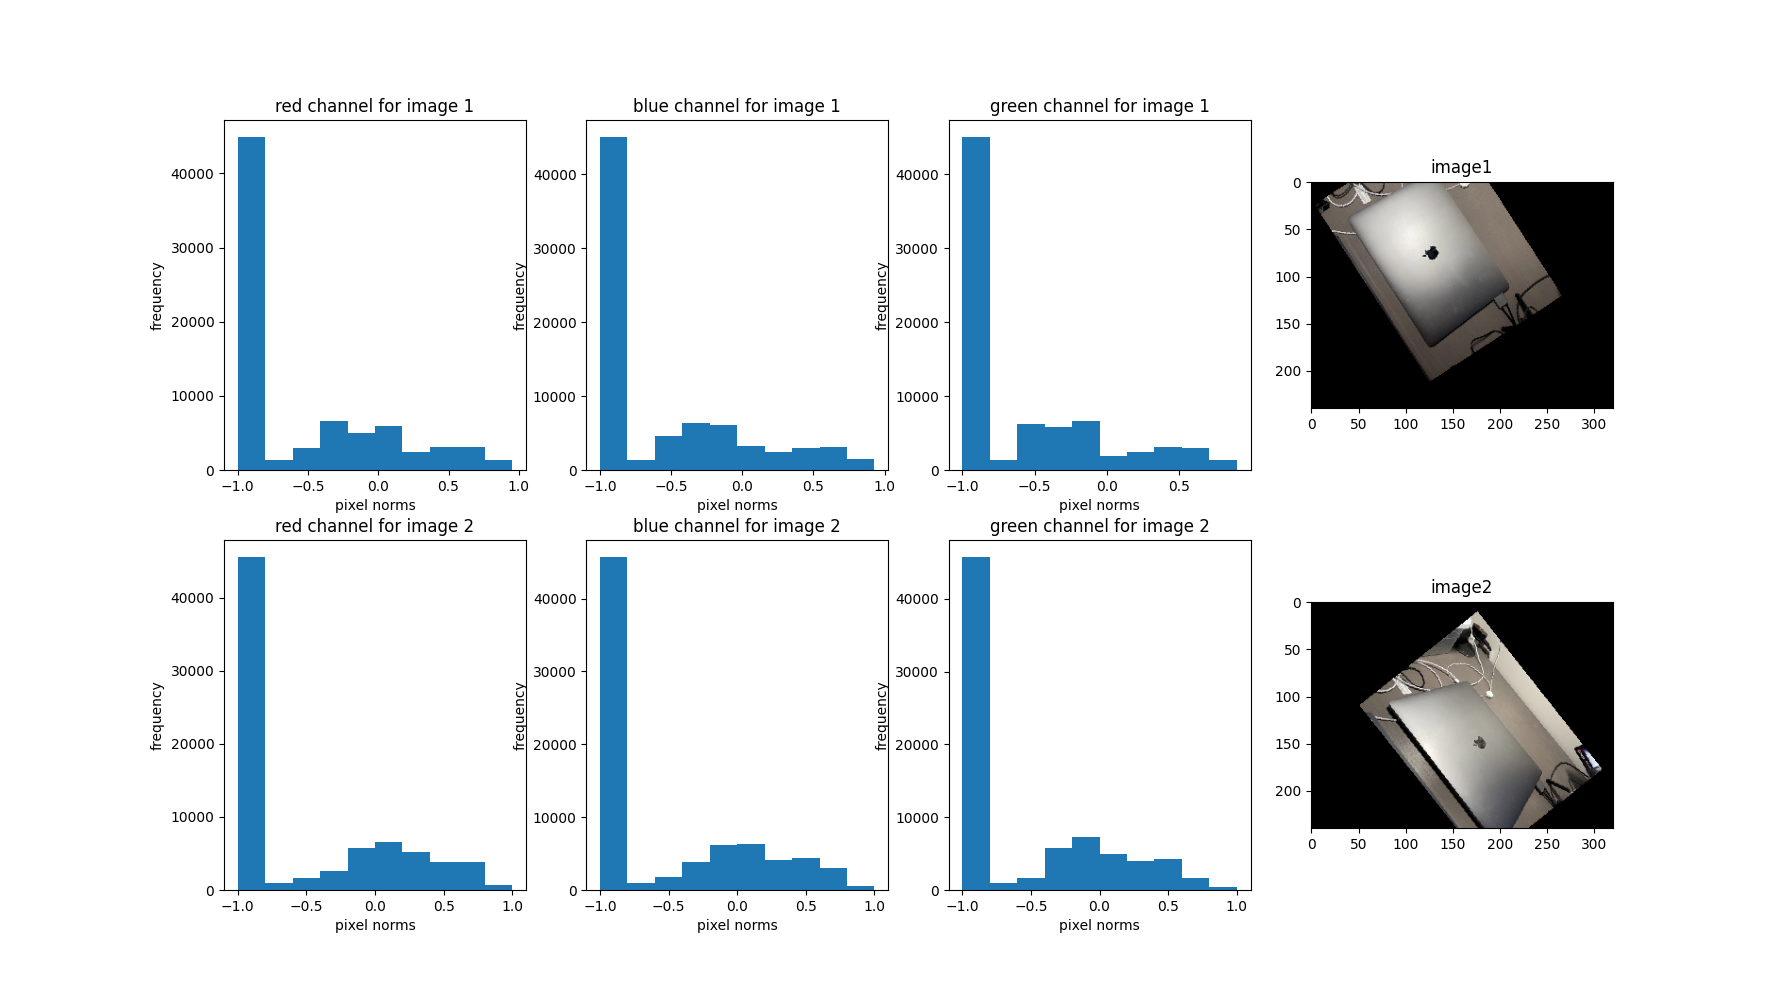
\includegraphics[scale=0.38]{2.png}\\
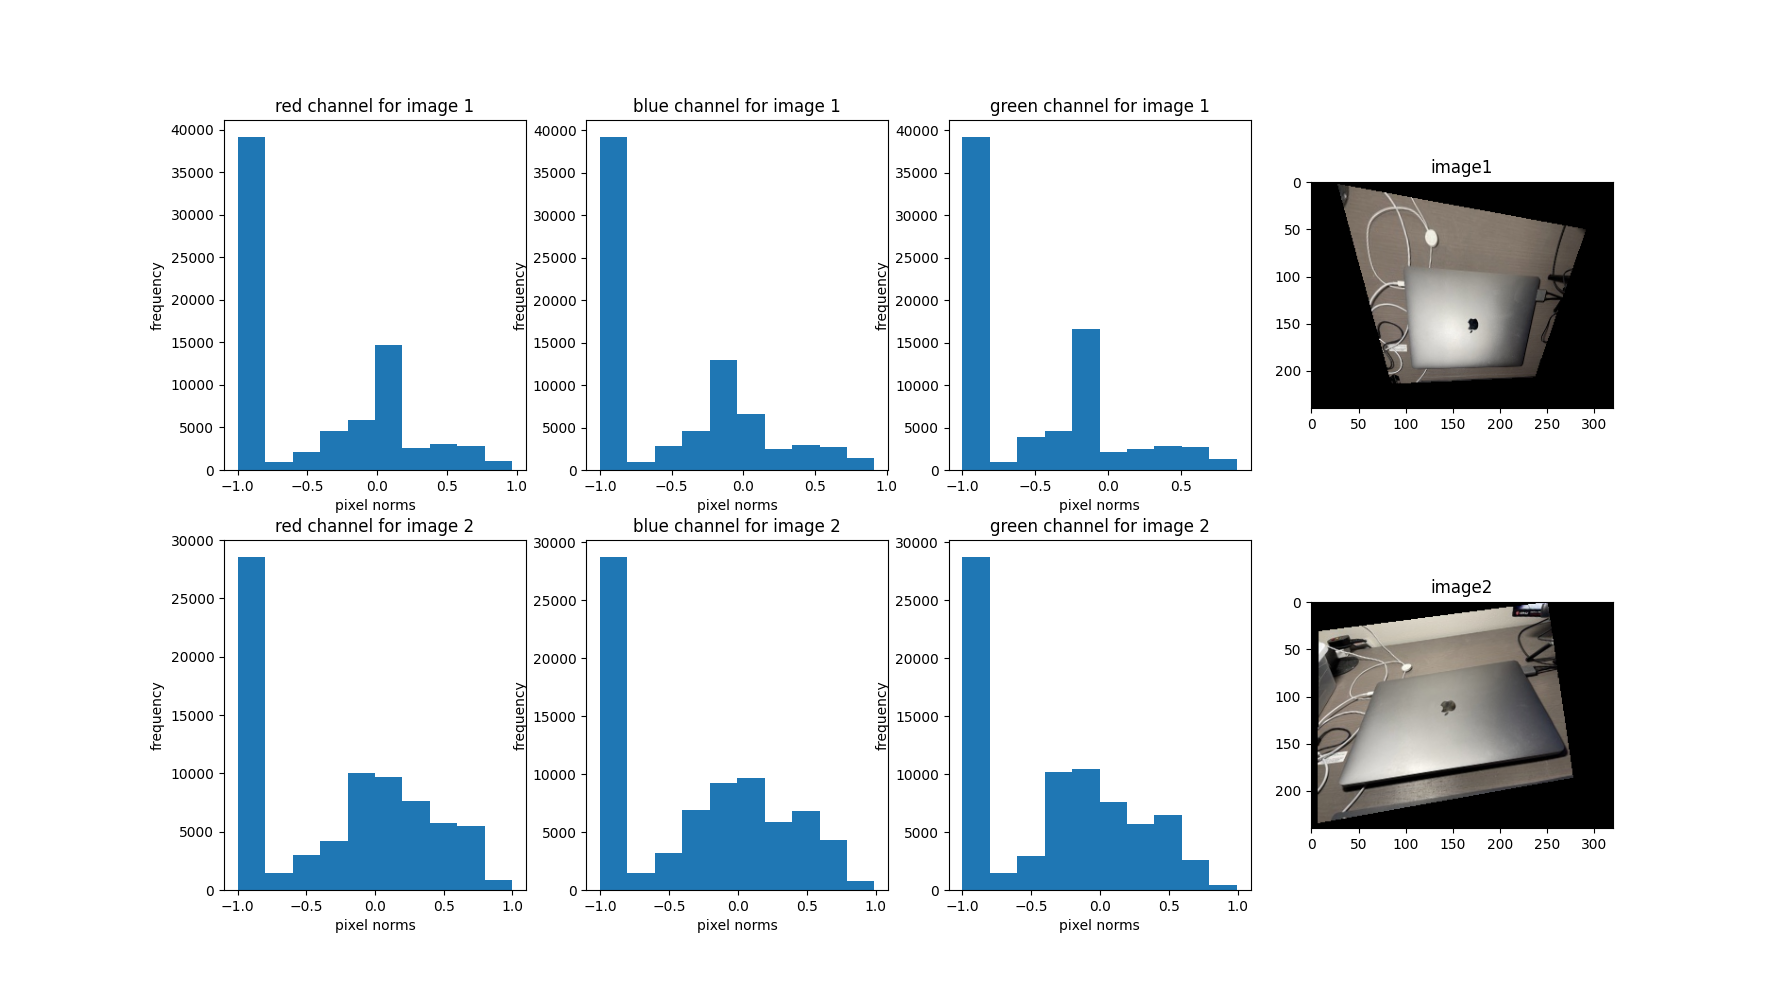
\includegraphics[scale=0.38]{3.png}
\subsection{printed distances}
0.014065103605389595 0.02574739586561918 0.017520831339061262\\
0.004164060857146979 0.005205726716667414 0.005460935877636075\\
0.008005207777023316 0.015411460027098655 0.014057292370125653

\textcolor{red}{\rule[-0.3in]{6.1in}{0.03in}}\\
\vspace{-0.05in}
\begin{verbatim}
from PIL import Image
from PIL import ImageFilter
from PIL import ImageFont
from PIL import ImageDraw
from PIL import ImageChops
#from PIL import ImageTk
import torchvision.transforms as tvt
import torch
import numpy as np
import matplotlib.pyplot as plt
from scipy.stats import wasserstein_distance


def task3_4func(im1,im2,im_t,im2_t):
#print hists and dists

#task 3
    r_tensor = im_t[0]
    g_tensor = im_t[1]
    b_tensor = im_t[2]

    hist_r = torch.histc(r_tensor, bins = 10, min = -1.0, max = 1.0)
    hist_g = torch.histc(g_tensor, bins = 10, min = -1.0, max = 1.0)
    hist_b = torch.histc(b_tensor, bins = 10, min = -1.0, max = 1.0)
    
    hist_r = hist_r.div(hist_r.sum())
    hist_g = hist_g.div(hist_g.sum())
    hist_b = hist_b.div(hist_b.sum())
    
    r2_tensor = im2_t[0]
    g2_tensor = im2_t[1]
    b2_tensor = im2_t[2]
    
    hist2_r = torch.histc(r2_tensor, bins = 10, min = -1.0, max = 1.0)
    hist2_g = torch.histc(g2_tensor, bins = 10, min = -1.0, max = 1.0)
    hist2_b = torch.histc(b2_tensor, bins = 10, min = -1.0, max = 1.0)

    hist2_r = hist2_r.div(hist2_r.sum())
    hist2_g = hist2_g.div(hist2_g.sum())
    hist2_b = hist2_b.div(hist2_b.sum())
    #print(hist_r.type(), hist_r.shape)
    
    fig, axs = plt.subplots(nrows = 2, ncols = 4, figsize = (20, 10))
    plt.subplot(2,4,1)
    plt.xlabel("pixel norms")
    plt.ylabel("frequency")
    plt.title("red channel for image 1")
    plt.hist(r_tensor.view(1,-1))
    plt.subplot(2,4,2)
    plt.xlabel("pixel norms")
    plt.ylabel("frequency")
    plt.title("blue channel for image 1")
    plt.hist(g_tensor.view(1,-1))
    plt.subplot(2,4,3)
    plt.xlabel("pixel norms")
    plt.ylabel("frequency")
    plt.title("green channel for image 1")
    plt.hist(b_tensor.view(1,-1))
    plt.subplot(2,4,4)
    plt.imshow(im1)
    plt.title("image1")
    
    plt.subplot(2,4,5)
    plt.xlabel("pixel norms")
    plt.ylabel("frequency")
    plt.title("red channel for image 2")
    plt.hist(r2_tensor.view(1,-1))
    plt.subplot(2,4,6)
    plt.xlabel("pixel norms")
    plt.ylabel("frequency")
    plt.title("blue channel for image 2")
    plt.hist(g2_tensor.view(1,-1))
    plt.subplot(2,4,7)
    plt.xlabel("pixel norms")
    plt.ylabel("frequency")
    plt.title("green channel for image 2")
    plt.hist(b2_tensor.view(1,-1))
    plt.subplot(2,4,8)
    plt.imshow(im2)
    plt.title("image2")
    plt.show()

# task 4

    dist_r = wasserstein_distance(torch.squeeze(hist_r).cpu().numpy(), torch.squeeze(hist2_r).cpu().numpy())
    dist_g = wasserstein_distance(torch.squeeze(hist_g).cpu().numpy(), torch.squeeze(hist2_g).cpu().numpy())
    dist_b = wasserstein_distance(torch.squeeze(hist_b).cpu().numpy(), torch.squeeze(hist2_b).cpu().numpy())
    print(dist_r, dist_g, dist_b) #0.014065103605389595 0.02574739586561918 0.017520831339061262 without transformation


if __name__ == "__main__":

#task 2
    im1 = Image.open("image1.jpeg")
    #print(im1.format, im1.size, im1.mode) #PNG (320, 240) RGBA
    im2 = Image.open("image2.jpeg")
    #print(im2.format, im2.size, im2.mode) #PNG (320, 240) RGBA

    xform = tvt.Compose([tvt.ToTensor(), tvt.Normalize([0.5, 0.5, 0.5], [0.5, 0.5, 0.5])])
    im_t = xform(im1)
    im2_t = xform(im2)
    task3_4func(im1,im2,im_t,im2_t)
#    print(im_t)
#    print(im2_t)
#    print(im_t.shape)


#task 5
#torchvision.transforms.RandomAffine(degrees, translate=None, scale=None, shear=None, resample=False, fillcolor=
    aff = tvt.RandomAffine(degrees = (30,70), translate = (0.1, 0.3), scale = (0.5, 0.75))

    im_af = aff(im1)
    im2_af = aff(im2)
    im_af_t = xform(im_af)
    im2_af_t = xform(im2_af)
    task3_4func(im_af,im2_af,im_af_t,im2_af_t)


#task 6
#torchvision.transforms.functional.perspective(img, startpoints, endpoints, interpolation=3)
    persp = tvt.RandomPerspective(distortion_scale=0.6, p=1.0)
    im_persp = persp(im1)
    im2_persp = persp(im2)
    im_persp_t = xform(im_persp)
    im2_persp_t = xform(im2_persp)
    task3_4func(im_persp, im2_persp, im_persp_t, im2_persp_t)
\end{verbatim}
\vspace{-0.45in}
\textcolor{red}{\rule[-0.3in]{6.1in}{0.03in}}\\

\section{Lessons Learned}
When working on this homework, lots of processes are the same to both images and to all three channels. I have to be careful with replacing the variable names.
\section{Suggested Enhancements}
For this homework, I would improve the pyplot coding part. There are lots of repeated coding that needs to improve.
\end{document}